% =====================================================================
%  CLASE 05 -- Acuíferos costeros, hidráulica de pozos en régimen
%              impermanente
% =====================================================================
\clase{05}{Acuíferos costeros e hidráulica de pozos en régimen impermanente}

\section{Acuíferos costeros: intrusión salina}

La intrusión salina se analiza como un \textbf{equilibrio estático de
columnas de agua de diferente densidad} (aproximación de Ghyben--Herzberg):
\begin{itemize}
  \item El flujo de agua dulce es perfectamente horizontal.
  \item No existe flujo de agua salada.
  \item La interfaz es un plano, no existiendo zona de mezcla.
\end{itemize}

\begin{figure}[H]
\centering
\begin{tikzpicture}[font=\small,scale=1.1]
  % agua subterránea dulce
  \fill[aguaclara] (0,0) -- (0.8,0) .. controls (2.5,0.5) and (4.5,1.6) .. (5.5,2.6)
     .. controls (4,2.85) and (2,3.1) .. (0,3.2) -- cycle;
  % agua subterránea salada
  \fill[azulusm!75] (0.8,0) .. controls (2.5,0.5) and (4.5,1.6) .. (5.5,2.6)
     .. controls (6.5,2.0) and (7.5,1.1) .. (9,0.8) -- (9,0) -- cycle;
  % mar
  \fill[azulusm!45] (5.5,2.6) .. controls (6.5,2.0) and (7.5,1.1) .. (9,0.8) -- (9,2.6) -- cycle;
  % zona no saturada
  \fill[gray!35] (0,3.2) .. controls (2,3.1) and (4,2.85) .. (5.5,2.6)
     .. controls (4,3.2) and (2,3.7) .. (0,3.8) -- cycle;
  \draw (0,3.8) .. controls (2,3.7) and (4,3.2) .. (5.5,2.6) .. controls (6.5,2.0) and (7.5,1.1) .. (9,0.8);
  \draw[thick,azulusm] (0,3.2) .. controls (2,3.1) and (4,2.85) .. (5.5,2.6);
  \draw (5.5,2.6) -- (9,2.6);
  \fill[pattern=north east lines] (0,-0.25) rectangle (9,0);
  \pic at (0.4,3.18) {nivelagua}; \pic at (8.6,2.62) {nivelagua};
  \draw[dashed] (0,2.6) -- (5.5,2.6);
  \draw[cota] (3.3,2.6) -- (3.3,2.93) node[midway,left]{$h_d$};
  \draw[cota] (3.3,1.25) -- (3.3,2.6) node[midway,left]{$h_s$};
  \draw[dashed] (3.3,1.25) -- (8.4,1.25);
  \draw[cota] (8.4,1.25) -- (8.4,2.6) node[midway,left]{$h_s$};
  \node at (0.5,2.2) {$\gamma_d$}; \node[align=center] at (1.2,1.4) {Agua\\dulce};
  \node at (8.7,1.0) {$\gamma_s$}; \node[align=center,white] at (6.0,0.6) {Agua\\salada};
  \node at (8.6,2.2) {Mar};
  \draw[<-] (5.5,2.65) -- (5.1,3.5) node[above left,azulusm]{Línea de costa};
  \draw[<-] (4.3,1.6) -- (7.6,3.4) node[above,azulusm]{Intrusión salina};
\end{tikzpicture}
\caption{Equilibrio de agua dulce y salada en un acuífero costero.}
\end{figure}

Las presiones sobre la interfaz son:
\[
P_d=\gamma_d\,(h_d+h_s),\qquad P_s=\gamma_s\,h_s
\]
Considerando $P_s=P_d$:
\begin{formula}
$\displaystyle h_s=h_d\left(\frac{\gamma_d}{\gamma_s-\gamma_d}\right)$
\end{formula}
Considerando que $\gamma_d=1000$ [kgf/m$^3$] y $\gamma_s=1025$ [kgf/m$^3$]:
\begin{formula}
$h_s=40\,h_d$
\end{formula}
La manera segura de evitar que un pozo entregue agua salada es que su
profundidad no pase el nivel del mar: al bombear, el descenso del nivel
de agua dulce provoca un ascenso de la interfaz 40 veces mayor
(\emph{upconing}).

\begin{nota}[title={Ejemplo: intrusión salina en una isla}]
Una isla de forma aproximadamente circular de 10 [km] de diámetro está
geológicamente constituida por suelos con $K=1\times10^{-4}$ [m/s]. La isla
recibe una recarga por infiltración de lluvias de aproximadamente 4 [mm/día],
formando un acuífero de agua dulce rodeado de agua salada de densidad
relativa $\gamma_{sr}=1.025$.
\begin{enumerate}[label=\alph*)]
  \item Estimar la cota sobre el nivel del mar a la que se encontrará la napa
        subterránea en su punto más alto en la isla.
  \item ¿A qué profundidad se hallará agua salada a 1 [km] de distancia de la costa?
\end{enumerate}
\end{nota}

\section{Ecuaciones generales (recordatorio)}
Conservación de la masa, flujo saturado:
\begin{formula}
$\displaystyle
\frac{\partial}{\partial x}\left(K_x\frac{\partial h}{\partial x}\right)+
\frac{\partial}{\partial y}\left(K_y\frac{\partial h}{\partial y}\right)+
\frac{\partial}{\partial z}\left(K_z\frac{\partial h}{\partial z}\right)=S_s\frac{\partial h}{\partial t}$
\end{formula}
Flujo transiente en medio homogéneo e isotrópico:
\[
\frac{\partial^2h}{\partial x^2}+\frac{\partial^2h}{\partial y^2}+\frac{\partial^2h}{\partial z^2}=\frac{S_s}{K}\frac{\partial h}{\partial t}
\]

\section{Acuíferos confinados: régimen transiente}

\begin{itemize}
  \item En un acuífero confinado el agua se obtiene del almacenamiento
        específico del acuífero, $S_s=S/b$, con $b$ el espesor del acuífero.
  \item En un acuífero confinado, $S$ es generalmente muy pequeño (0.005 o
        menos), entonces el bombeo afecta un área relativamente extensa del acuífero.
  \item Acuífero horizontal, confinado en la base y techo. Sin fuente de recarga.
  \item Los coeficientes $K$, $S$ son constantes e independientes del tiempo
        durante el bombeo.
  \item Caudal de bombeo a tasa constante, sin llegar a régimen permanente.
  \item El agua de almacenamiento se moviliza hacia el pozo de bombeo
        inmediatamente después de producirse las depresiones de la napa (el
        agua se libera instantánea e inmediatamente a la extracción).
  \item En el caso del régimen transiente (no se alcanza la estabilización del
        cono), cuando se indica un $Q$ de extracción se debe hacer referencia
        al tiempo desde que se inicia el bombeo.
\end{itemize}
\textcolor{rojo}{Estamos resolviendo el sistema para una distancia radial $r$
del pozo de extracción, de modo que ahora la altura piezométrica variará en
el tiempo y en el espacio (no se alcanza el equilibrio).}

% Macro: pozo en régimen transiente
\newcommand{\pozotransiente}[1]{% #1 = 1 confinado, 0 libre
\begin{tikzpicture}[font=\small,scale=0.9]
  \draw[thick] (-4,0) -- (4,0);
  \foreach \x in {-3.9,-3.6,...,3.9} \draw (\x,0) -- (\x-0.2,-0.25);
  \draw[thick] (-0.4,0.05) -- (-0.4,4.4) (0.4,0.05) -- (0.4,4.4);
  \draw[thick] (-4,4.4) -- (-0.4,4.4) (0.4,4.4) -- (4,4.4);
  \fill[azulusm] (-0.1,4.2) rectangle (0.1,4.9);
  \fill[azulusm] (-0.25,4.9) -- (0.25,4.9) -- (0,5.25) -- cycle; \node at (0.55,5.1) {$Q$};
  \draw[cyan!70!blue,thick] (-4,3.6) -- (-0.4,3.6) (0.4,3.6) -- (4,3.6);
  \node[left] at (-4,3.6) {$t=0$};
  \draw[dashed,cyan!70!blue,thick] (-4,3.1) .. controls (-2,2.9) and (-1,2.6) .. (-0.4,2.3);
  \draw[dashed,cyan!70!blue,thick] (0.4,2.3) .. controls (1,2.6) and (2,2.9) .. (4,3.1);
  \draw[cyan!70!blue,thick] (-0.4,2.3) -- (0.4,2.3);
  \node[left] at (-4,3.1) {$t=t$};
  \ifnum#1=1
    \draw[thick] (-4,2.0) -- (-0.4,2.0) (0.4,2.0) -- (4,2.0);
    \foreach \x in {-3.9,-3.6,...,-0.6,0.6,0.9,...,3.9} \draw (\x,2.0) -- (\x+0.15,2.25);
    \draw[cota] (-3.3,0) -- (-3.3,2.0) node[midway,left]{$m$};
    \def\ytop{1.8}
  \else
    \def\ytop{2.0}
  \fi
  \foreach \y in {0.3,0.6,...,\ytop}{\draw[->,azulusm] (-1.3,\y) -- (-0.5,\y);\draw[->,azulusm] (1.3,\y) -- (0.5,\y);}
  \node[right] at (1.3,1.0) {$Q_i$};
  \draw[cota] (-2.3,0) -- (-2.3,3.6) node[midway,right]{$H$};
  \draw[cota] (2.8,0) -- (2.8,2.95) node[midway,right]{$h(r,t)$};
  \draw[->] (0,-0.5) -- (2.8,-0.5) node[midway,below]{$r$};
\end{tikzpicture}}

\begin{figure}[H]
\centering
\pozotransiente{1}
\caption{Pozo en acuífero confinado en régimen transiente.}
\end{figure}

\subsection{Solución de Theis (1935)}
Hipótesis: acuífero horizontal, confinado entre formaciones impermeables, de
extensión horizontal infinita, espesor constante, homogéneo e isotrópico,
pozo de radio infinitesimalmente pequeño. Se asume además que $Q_i=Q_s$ (no
hay acumulación en el pozo), lo que se cumple si el radio del pozo es pequeño.

En coordenadas cilíndricas:
\begin{formula}
$\displaystyle\frac{\partial^2h}{\partial r^2}+\frac1r\frac{\partial h}{\partial r}=\frac ST\frac{\partial h}{\partial t}$
\end{formula}
La solución de Theis es:
\begin{formula}
$\displaystyle\Delta h(r,t)=H-h(r,t)=\frac{Q}{4\pi T}W(u),\qquad
W(u)=\int_u^\infty\frac{e^{-u}}{u}\,\dd u,\qquad u=\frac{r^2\cdot S}{4\cdot T\cdot t}$
\end{formula}
$W(u)$ es conocida como la \textbf{función del pozo} (\emph{well function}):
\[
W(u)=\int_u^\infty\frac{e^{-u}}{u}\,\dd u=-0.577216-\ln u+u-\frac{u^2}{2\cdot2!}+\frac{u^3}{3\cdot3!}-\dots
\]

\subsection{Aproximación de Cooper--Jacob (1946)}
Si $r$ es pequeño ($u<0.01$) y $t\to\infty$, basta con los dos primeros
términos de la serie:
\begin{formula}
$\displaystyle H-h(r,t)\approx\frac{Q}{4\pi T}\ln\left(\frac{2.24\cdot T\cdot t}{S\cdot r^2}\right)$\qquad\textbf{Cooper--Jacob (1946)}
\end{formula}
\begin{table}[H]
\centering
\begin{tabular}{cc}
\toprule
$u$ & Error\\
\midrule
0.20 & 20\%\\
0.14 & 10\%\\
0.09 & 5\%\\
\bottomrule
\end{tabular}
\caption{Error de la aproximación de Cooper--Jacob.}
\end{table}
De este modo, conociendo las características hidrogeológicas ($S$, $T$), se
puede estimar el descenso en cualquier parte del acuífero, una vez iniciado el bombeo.

\subsection{Función del pozo, $W(u)$}
\begin{figure}[H]
\centering
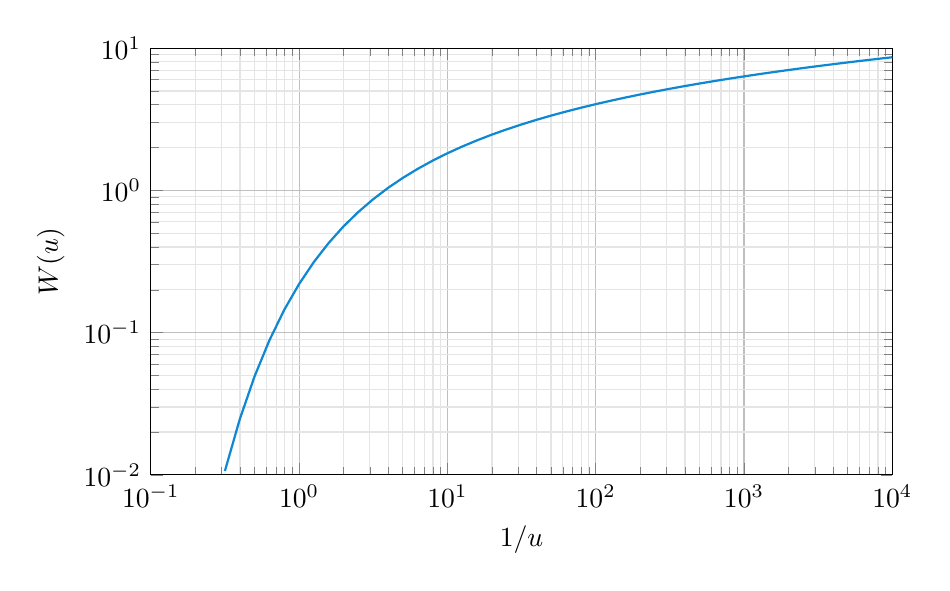
\begin{tikzpicture}
\begin{loglogaxis}[width=11cm,height=7cm,xmin=0.1,xmax=1e4,ymin=0.01,ymax=10,
  xlabel={$1/u$},ylabel={$W(u)$},grid=both,minor grid style={gray!20},major grid style={gray!50}]
\addplot[thick,cyan!70!blue] coordinates {(0.3162,0.01063) (0.3981,0.02453) (0.5012,0.04922) (0.631,0.08824) (0.7943,0.1444) (1,0.2194) (1.259,0.3138) (1.585,0.4272) (1.995,0.5583) (2.512,0.7056) (3.162,0.867) (3.981,1.041) (5.012,1.225) (6.31,1.417) (7.943,1.617) (10,1.823) (12.59,2.034) (15.85,2.248) (19.95,2.466) (25.12,2.686) (31.62,2.908) (39.81,3.132) (50.12,3.357) (63.1,3.583) (79.43,3.81) (100,4.038) (125.9,4.266) (158.5,4.495) (199.5,4.724) (251.2,4.953) (316.2,5.182) (398.1,5.412) (501.2,5.642) (631,5.872) (794.3,6.102) (1000,6.332) (1259,6.562) (1585,6.792) (1995,7.022) (2512,7.252) (3162,7.482) (3981,7.712) (5012,7.943) (6310,8.173) (7943,8.403) (1e+04,8.633)};
\end{loglogaxis}
\end{tikzpicture}
\caption{Curva tipo de Theis: $W(u)$ versus $1/u$.}
\end{figure}

\begin{table}[H]
\centering\footnotesize
\begin{tabular}{c|ccccc}
\toprule
$N$ & $N\times10^{-14}$ & $N\times10^{-13}$ & $N\times10^{-12}$ & $N\times10^{-11}$ & $N\times10^{-10}$\\
\midrule
1 & 31.66 & 29.36 & 27.05 & 24.75 & 22.45\\
2 & 30.97 & 28.66 & 26.36 & 24.06 & 21.76\\
3 & 30.56 & 28.26 & 25.96 & 23.65 & 21.35\\
4 & 30.27 & 27.97 & 25.67 & 23.36 & 21.06\\
5 & 30.05 & 27.75 & 25.44 & 23.14 & 20.84\\
6 & 29.87 & 27.56 & 25.26 & 22.96 & 20.66\\
7 & 29.71 & 27.41 & 25.11 & 22.81 & 20.50\\
8 & 29.58 & 27.28 & 24.97 & 22.67 & 20.37\\
9 & 29.46 & 27.16 & 24.86 & 22.55 & 20.25\\
\bottomrule
\end{tabular}\par\medskip
\begin{tabular}{c|ccccc}
\toprule
$N$ & $N\times10^{-9}$ & $N\times10^{-8}$ & $N\times10^{-7}$ & $N\times10^{-6}$ & $N\times10^{-5}$\\
\midrule
1 & 20.15 & 17.84 & 15.54 & 13.24 & 10.94\\
2 & 19.45 & 17.15 & 14.85 & 12.55 & 10.24\\
3 & 19.05 & 16.74 & 14.44 & 12.14 & 9.84\\
4 & 18.76 & 16.46 & 14.15 & 11.85 & 9.55\\
5 & 18.54 & 16.23 & 13.93 & 11.63 & 9.33\\
6 & 18.35 & 16.05 & 13.75 & 11.45 & 9.14\\
7 & 18.20 & 15.90 & 13.59 & 11.29 & 8.99\\
8 & 18.07 & 15.76 & 13.46 & 11.16 & 8.86\\
9 & 17.95 & 15.65 & 13.34 & 11.04 & 8.74\\
\bottomrule
\end{tabular}\par\medskip
\begin{tabular}{c|ccccc}
\toprule
$N$ & $N\times10^{-4}$ & $N\times10^{-3}$ & $N\times10^{-2}$ & $N\times10^{-1}$ & $N\times10^{0}$\\
\midrule
1 & 8.63 & 6.33 & 4.04 & 1.82 & 0.22\\
2 & 7.94 & 5.64 & 3.35 & 1.22 & $4.9\times10^{-2}$\\
3 & 7.53 & 5.23 & 2.96 & 0.91 & $1.3\times10^{-2}$\\
4 & 7.25 & 4.95 & 2.68 & 0.70 & $3.8\times10^{-3}$\\
5 & 7.02 & 4.73 & 2.47 & 0.56 & $1.1\times10^{-3}$\\
6 & 6.84 & 4.54 & 2.30 & 0.45 & $3.6\times10^{-4}$\\
7 & 6.69 & 4.39 & 2.15 & 0.37 & $1.2\times10^{-4}$\\
8 & 6.55 & 4.26 & 2.03 & 0.31 & $3.8\times10^{-5}$\\
9 & 6.44 & 4.14 & 1.92 & 0.26 & $1.2\times10^{-5}$\\
\bottomrule
\end{tabular}\par\medskip
\caption{Valores de la función del pozo $W(u)$ para $u=N\times10^{k}$.}
\end{table}

\subsection{Radio de influencia dependiente del tiempo}
En equilibrio: $\displaystyle\Delta h=\frac{Q}{2\pi T}\ln\left(\frac Rr\right)$.
A partir de Cooper--Jacob se define:
\begin{formula}
$\displaystyle R(t)=\sqrt{\frac{2.24\cdot T\cdot t}{S}}
\quad\Longrightarrow\quad
\Delta h=\frac{Q}{2\pi T}\ln\left(\frac{R(t)}{r}\right)$\qquad (desequilibrio)
\end{formula}

\section{Acuíferos libres: régimen transiente}
Ecuación gobernante:
\[
2\frac hr\frac{\partial h}{\partial r}+\frac{\partial^2h}{\partial r^2}=\frac{S}{K\cdot h}\frac{\partial h}{\partial t}
\]
Siguiendo el resultado del caso confinado, se establece la analogía
(en equilibrio $H^2-h^2=\frac{Q}{\pi K}\ln\frac Rr$):
\begin{formula}
$\displaystyle R(t)=\sqrt{\frac{2.24\cdot T\cdot t}{S}}\quad\Longrightarrow\quad
H^2-h(r,t)^2=\frac{Q}{\pi K}\ln\left(\frac{R(t)}{r}\right)$\qquad (desequilibrio)
\end{formula}

\begin{figure}[H]
\centering
\pozotransiente{0}
\caption{Pozo en acuífero libre en régimen transiente.}
\end{figure}

\section{Interferencia de pozos: régimen impermanente}
\paragraph{Depresión producto de múltiples pozos.} Similar a régimen
permanente $\Rightarrow$ solución: superposición.
\begin{formula}
$\displaystyle\Delta h_T=\sum_{i=1}^n\Delta h_i(r_i)$
\end{formula}
Siempre que $R(t)>r_i$. Esta restricción define el concepto de
\textbf{tiempo de influencia} ($t_i$):
\[
R(t)=\sqrt{\frac{2.24\cdot T\cdot t_i}{S}}=r_i\quad\Longrightarrow\quad
\boxed{t_i=\frac{r_i^2\cdot S}{2.24\cdot T}}
\]

Usando la solución de Jacob (acuíferos confinados):
\begin{itemize}
  \item Si todos los pozos afectan al punto ``A'':
  \begin{formula}
  $\displaystyle\Delta h_A=\sum_{i=1}^n\frac{Q_i}{4\cdot\pi\cdot T}\ln\left(\frac{2.24\cdot T\cdot t}{r_{i-A}^2\cdot S}\right),
  \qquad r_{i-A}\leq\sqrt{\frac{2.24\cdot T\cdot t}{S}}$
  \end{formula}
  \item Si todos los pozos extraen el mismo caudal:
  \begin{formula}
  $\displaystyle\Delta h_A=Q\sum_{i=1}^n\frac{1}{4\cdot\pi\cdot T}\ln\left(\frac{2.24\cdot T\cdot t}{r_{i-A}^2\cdot S}\right),
  \qquad r_{i-A}\leq\sqrt{\frac{2.24\cdot T\cdot t}{S}}$
  \end{formula}
  \item ¡Para acuíferos libres, linealizar primero!
\end{itemize}

\section{Método de las imágenes en régimen impermanente}
Superposición de soluciones para obtener la respuesta a condiciones de borde
específicas: recargas lineales (masas de agua con nivel constante) y barreras
impermeables. Es similar a régimen permanente, pero se debe tener en cuenta
el tiempo $t$ en el que se toma la medición y los tiempos de influencia de
los pozos ($t_r$: pozo real, $t_i$: pozo imagen).

\paragraph{Recarga lineal}
\begin{itemize}
  \item Si $t_r<t<t_i$:\quad $\displaystyle\Delta h_T=\Delta h_{real}=\frac{Q}{2\pi T}\ln\left(\frac{R(t)}{r_r}\right)$
  \item Si $t>t_i$:\quad $\Delta h_T=\Delta h_{real}-\Delta h_{imag}$
  \begin{formula}
  $\displaystyle\Delta h_T=\frac{Q}{2\pi T}\ln\left(\frac{r_i}{r_r}\right)$
  \end{formula}
\end{itemize}

\paragraph{Barrera impermeable}
\begin{itemize}
  \item Si $t_r<t<t_i$:\quad $\displaystyle\Delta h_T=\Delta h_{real}=\frac{Q}{2\pi T}\ln\left(\frac{R(t)}{r_r}\right)$
  \item Si $t>t_i$:\quad $\Delta h_T=\Delta h_{real}+\Delta h_{imag}$
  \begin{formula}
  $\displaystyle\Delta h_T=\frac{Q}{2\pi T}\ln\left(\frac{R(t)^2}{r_r\cdot r_i}\right)$
  \end{formula}
\end{itemize}

\section{Bombeo variable}
Usando la solución de Jacob (acuíferos confinados), un bombeo intermitente
se descompone como la superposición de pozos que se encienden ($+Q$) y se
apagan ($-Q$) en los instantes $t_i$.

\begin{figure}[H]
\centering
\begin{tikzpicture}[font=\small]
  \begin{scope}[yshift=3.2cm]
    \draw[flecha] (0,0) -- (6.5,0) node[below]{$t$};
    \draw[flecha] (0,0) -- (0,2.2) node[left]{$Q$};
    \foreach \a in {0,2,4} \fill[azulusm!80] (\a,0) rectangle (\a+1,1.5);
    \node[left] at (0,1.5) {$Q_1$};
    \foreach \x/\n in {1/1,2/2,3/3,4/4,5/5} \node[below] at (\x,0) {$t_\n$};
  \end{scope}
  \draw[flecha] (0,0) -- (6.5,0) node[below]{$t$};
  \draw[flecha] (0,-1.8) -- (0,2.4) node[left]{$Q$};
  \draw[azulusm,very thick] (0,0.5) -- (6,0.5); \node[left] at (0,0.5) {$Q_1$};
  \draw[azulusm,very thick] (2,1.1) -- (6,1.1); \node[left] at (2,1.1) {$Q_1$};
  \draw[azulusm,very thick] (4,1.7) -- (6,1.7); \node[left] at (4,1.7) {$Q_1$};
  \draw[gray,very thick] (1,-0.5) -- (6,-0.5); \node[left] at (1,-0.5) {$-Q_1$};
  \draw[gray,very thick] (3,-1.0) -- (6,-1.0); \node[left] at (3,-1.0) {$-Q_1$};
  \draw[gray,very thick] (5,-1.5) -- (6,-1.5); \node[left] at (5,-1.5) {$-Q_1$};
  \foreach \x in {1,2,3,4,5} \draw[dashed,gray] (\x,-1.6) -- (\x,3.2);
\end{tikzpicture}
\caption{Bombeo intermitente descompuesto en pozos ficticios que se encienden y apagan.}
\end{figure}

Por lo tanto,
\[
\Delta h=\sum\Delta h_i=\frac{1}{4\cdot\pi\cdot T}\sum_{i=1}^n\pm Q\cdot\ln\left(\frac{2.24\cdot T}{r^2\cdot S}(t-t_i)\right),
\qquad\text{para } t\geq t_i
\]
Generalizando:
\begin{formula}
$\displaystyle\Delta h=\sum\Delta h_i=\frac{1}{4\cdot\pi\cdot T}\sum_{i=1}^n\pm Q_i\cdot\ln\left(\frac{2.24\cdot T}{r^2\cdot S}(t-t_i)\right),
\qquad t\geq t_i$
\end{formula}
